\section{Let's Emphasize \emph{Connectivity}}
We propose a novel connectivity-preserving metric to evaluate tubular and linear structure segmentation based on intersecting skeletons with masks. We call this metric \textit{centerlineDice} or \textbf{\textit{clDice}}.
\begin{figure*}[]
\begin{center}
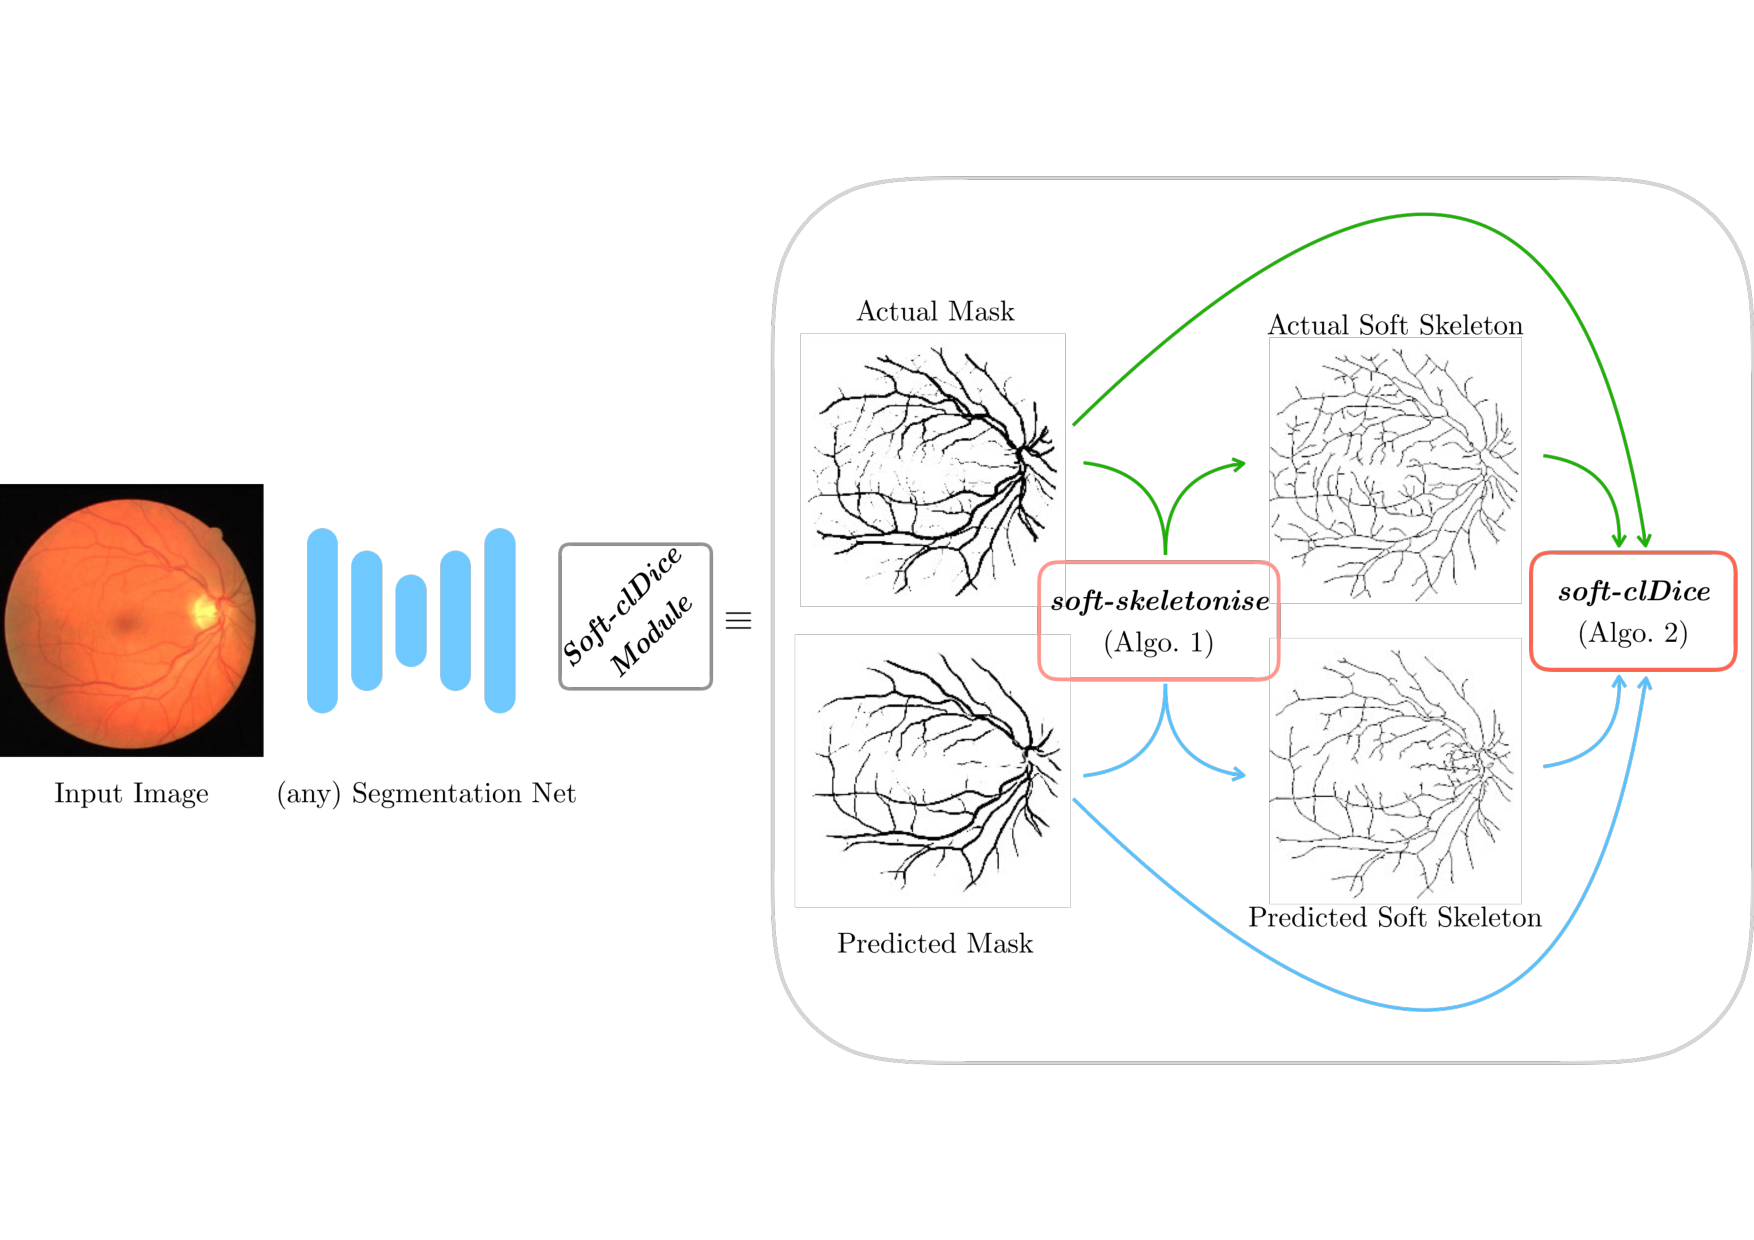
\includegraphics[width=0.85\textwidth]{figs/overview.pdf}
\end{center}
\label{met}
\caption{ \textbf{Schematic overview of our proposed method:} Our proposed \textit{clDice} loss can be applied to any arbitrary segmentation network. The soft-skeletonization can be easily implemented using pooling functions from any standard deep-learning toolbox.}
\vspace{-1em}
\end{figure*}

We consider two binary masks: the ground truth mask ($V_L$) and the predicted segmentation masks ($V_P$). First, the skeletons $ S_P$ and $ S_L$ are extracted from $V_P$ and $V_L$ respectively. Subsequently, we compute the fraction of $S_P$ that lies within $V_L$, which we call \textit{Topology Precision} or $\operatorname{Tprec}(S_P, V_L)$, and vice-a-versa we obtain \textit{Topology Sensitivity} or $\operatorname{Tsens}(S_L, V_P)$ as defined bellow;
\begin{align}
\operatorname{Tprec}(S_P, V_L) = \frac{|S_P  \cap V_L|}{|S_P|};~~
\operatorname{Tsens}(S_L, V_P) = \frac{|S_L  \cap V_P|}{|S_L|}\label{top_def}
\end{align}
We observe that the measure $\operatorname{Tprec}(S_P, V_L)$ is susceptible to false positives in the prediction while the measure $\operatorname{Tsens}(S_L, V_P)$ is susceptible to false negatives. This explains our rationale behind referring to the $\operatorname{Tprec}(S_P, V_L)$ as topology's precision and to the $\operatorname{Tsens}(S_L, V_P)$ as its sensitivity. Since we want to maximize both precision and sensitivity (recall), we define \textit{clDice} to be the harmonic mean (also known as F1 or Dice) of both the measures:
\begin{align}
\operatorname{clDice}(V_P, V_L) & = 2 \times \dfrac{ \operatorname{Tprec}(S_P, V_L) \times \operatorname{Tsens}(S_L, V_P)}{\operatorname{Tprec}(S_P, V_L) + \operatorname{Tsens}(S_L, V_P)}\label{eq2}
\end{align}
Note that our \textit{clDice} formulation is not defined for $\operatorname{Tprec} = 0 \mbox{ and } \operatorname{Tsens} = 0$, but can easily be extended continuously with the value $0$.